\documentclass[11pt]{article}

\usepackage{amsmath}
\usepackage{amssymb}
\usepackage[margin=0.68in]{geometry}
\usepackage{booktabs}
\usepackage{enumitem}
\usepackage{fancyhdr}
\usepackage{graphicx}
\usepackage[table]{xcolor}
\usepackage[hidelinks]{hyperref}
\usepackage{listings}
\usepackage{microtype}
\usepackage{tabularx}
\usepackage{titlesec}
\graphicspath{{docs/lessons/assets/}{../assets/}}

\definecolor{Ink}{gray}{0}
\definecolor{CodeGray}{gray}{0.96}
\hypersetup{
  pdftitle={ADK Lesson 029: Inert Cue Scheduling and Audit},
  pdfauthor={Kevin Shanahan},
  pdfsubject={Deterministic cue timing, explicit confirmation, inert LED evidence, and bounded replay records},
  pdflang={en-US}
}
\pagestyle{fancy}
\fancyhf{}
\lhead{\textsc{ADK Lesson 029}}
\rhead{Inert Cue Scheduling and Audit}
\cfoot{\thepage}
\setlength{\headheight}{14pt}
\setlength{\parindent}{0pt}
\setlength{\parskip}{5pt}
\setlist{nosep,leftmargin=1.45em}
\titleformat{\section}{\Large\bfseries\color{Ink}}{\thesection}{0.5em}{}
\titleformat{\subsection}{\large\bfseries\color{Ink}}{\thesubsection}{0.5em}{}
\lstdefinestyle{adkcpp}{
  language=C++,
  backgroundcolor=\color{CodeGray},
  basicstyle=\ttfamily\small,
  keywordstyle=\color{Ink}\bfseries,
  commentstyle=\color{Ink},
  columns=fullflexible,
  keepspaces=true,
  showstringspaces=false,
  frame=single,
  rulecolor=\color{Ink},
  breaklines=true,
  tabsize=4
}
\newcommand{\checkbox}{\(\square\)}
\newcommand{\blank}[1]{\rule{#1}{0.4pt}}
\newcommand{\lessonbox}[1]{%
  \begin{center}\fcolorbox{Ink}{white}{\parbox{0.92\linewidth}{#1}}\end{center}}

\begin{document}

\begin{center}
  {\Huge\bfseries Inert Cue Scheduling and Audit}\\[4pt]
  {\Large Supply time, confirm explicitly, preserve every decision}\\[8pt]
  \textit{Opaque visual labels; no external action seam}
\end{center}

\begin{tabularx}{\linewidth}{@{}>{\bfseries}l X >{\bfseries}l X@{}}
Lesson & 029 --- component & Time & 180--240 minutes\\
Prerequisites & Lessons 001, 002, 011, 017 & Board & Arduino Mega 2560\\
Evidence & cue LEDs, state cadence, TP29, audit & Status & host verified; bench open\\
Energy class & E1: USB, passive buttons, resistor-limited LEDs\\
\end{tabularx}

\lessonbox{\textbf{Boundary.} Cue IDs are opaque visual labels. They do not
name pins, addresses, frequencies, launcher channels, or external equipment.
This lesson has no relay, transistor-driven load, initiator, radio, captured
protocol, generic callback, or output adapter. Confirmation is instructional
redundancy, not a safety interlock.}

\section{Mission and evidence chain}

\[
\text{plan + supplied time + review/confirm}
\rightarrow\text{snapshot}\rightarrow\text{inert LEDs + bounded audit}.
\]

The core receives values and returns values. Only the canonical example owns
the supported low-voltage indicators.

\subsection{Learning outcomes}

\begin{itemize}
  \item validate a fixed plan without allocation or a hidden clock;
  \item explain epoch-based offsets and confirmation-time visibility;
  \item distinguish Waiting, Confirmation, Active, Held, and terminal phases;
  \item preserve delayed decisions in an append-only audit;
  \item replay byte-stable records without treating Serial as proof;
  \item separate acquisition, active presentation, shutdown, and physical
        power removal.
\end{itemize}

\section{Orientation and unpowered inspection}

\begin{center}
% ADK visual: pencil
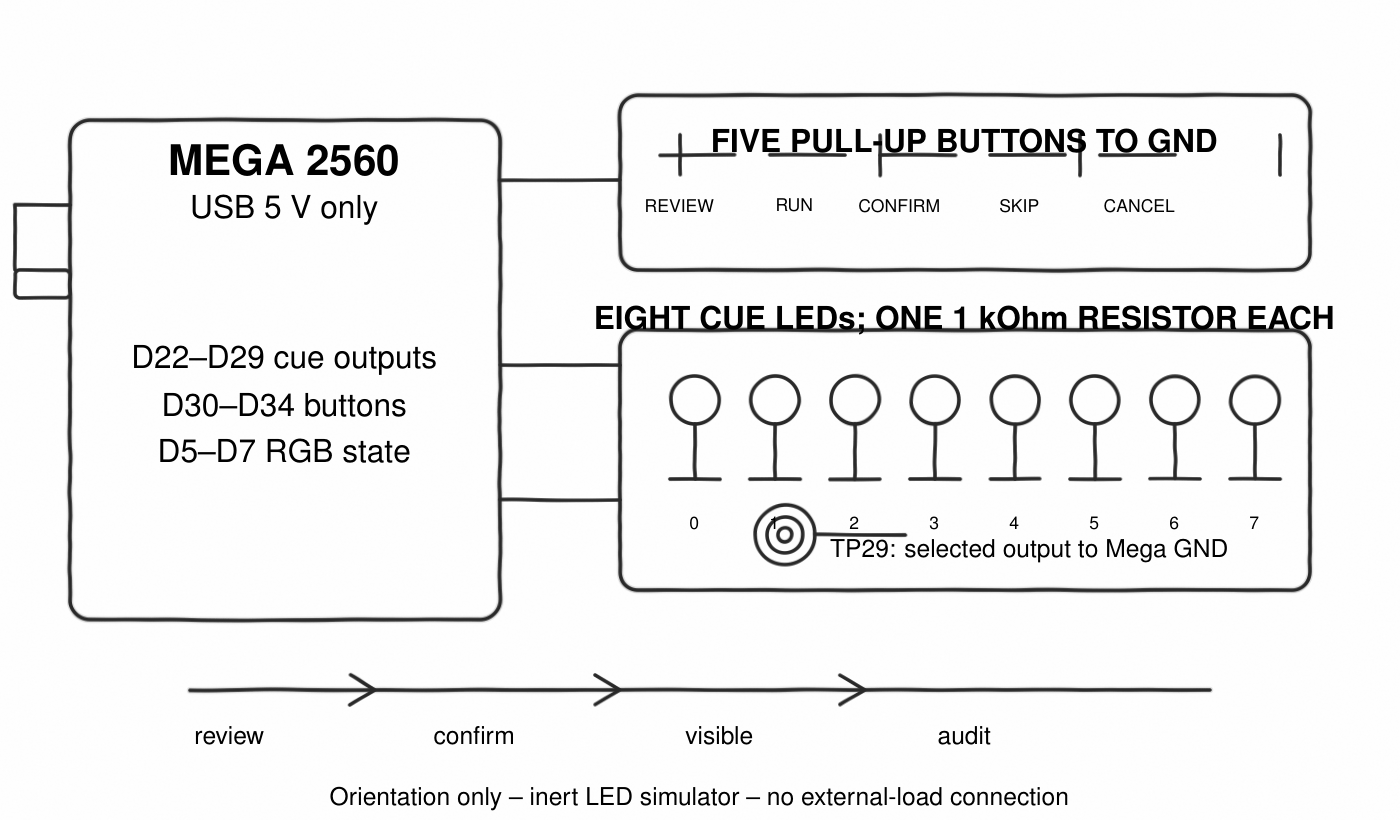
\includegraphics[width=0.96\linewidth]{029-inert-cue-pencil.png}

\small\textit{Alternative text: orientation plate showing one USB-powered
Mega, five pull-up buttons on D30--D34, eight separately resistor-limited cue
LEDs on D22--D29, a separately resistor-limited common-cathode RGB state LED on
D5--D7, and TP29 at the selected cue output. No external-load connection is
present.}
\end{center}

\begin{tabularx}{\linewidth}{@{}l l X@{}}
\toprule
Role & Mega pin & Connection\\
\midrule
cue indicators & D22--D29 & pin to 1 k\(\Omega\), LED anode; cathode to GND\\
operator controls & D30--D34 & Review, Run, Confirm, Skip, Cancel to GND; pull-up\\
RGB state & D5--D7 & red, green, blue through separate 1 k\(\Omega\) resistors\\
Lesson 029 TP29 & selected cue output & Mega-pin side of resistor, relative to GND\\
\bottomrule
\end{tabularx}

\textbf{Unpowered prediction.} Verify polarity, one resistor per LED channel,
five switch-to-ground paths, common ground, and no connection outside the
USB-powered fixture. Record resistor values: \blank{1.5in}.

\section{Current and resource worksheet}

The sketch commands at most one cue channel and one RGB channel. A deliberately
conservative zero-forward-voltage bound gives
\[
I_{\mathrm{channel}}\leq\frac{5.0\ \mathrm{V}}{1000\ \Omega}=5.0\ \mathrm{mA},
\qquad I_{\mathrm{LED,total}}\leq10.0\ \mathrm{mA}.
\]
This is a design bound, not a bench measurement.

\begin{tabularx}{\linewidth}{@{}X l l l X@{}}
\toprule
Quantity & Predicted & Measured & Calculated & Interpretation\\
\midrule
USB/5 V rail & at most 5.0 V & \blank{.7in} & --- & \blank{1.0in}\\
selected cue resistor & 1 k\(\Omega\) & \blank{.7in} & \(I=(V-V_f)/R\) & \blank{1.0in}\\
active RGB resistor & 1 k\(\Omega\) & \blank{.7in} & \(I=(V-V_f)/R\) & \blank{1.0in}\\
worst simultaneous LED load & at most 10 mA & \blank{.7in} & \blank{.8in} & \blank{1.0in}\\
\bottomrule
\end{tabularx}

D5--D7 use PWM-capable pins, but the example selects one fixed channel at a
time. D22--D34 are ordinary digital endpoints. No bus, interrupt, radio, motor,
or external supply is acquired.

\section{Plan and scheduler contract}

A valid plan contains 1--32 cues. IDs are unique values 0--31, offsets strictly
increase, visible durations are nonzero, active intervals do not overlap, and
the plan end stays inside the unambiguous half of 32-bit time.

\begin{tabularx}{\linewidth}{@{}l r r X@{}}
\toprule
Opaque ID & Offset & Visible for & Canonical display position\\
\midrule
3 & 2000 ms & 2000 ms & cue LED index 0\\
7 & 7000 ms & 2000 ms & cue LED index 1\\
12 & 12000 ms & 2000 ms & cue LED index 2\\
29 & 17000 ms & 2000 ms & cue LED index 3\\
\bottomrule
\end{tabularx}

Run establishes the plan epoch. Later offsets never move when confirmation is
late. A cue becomes visible at accepted confirmation and stays visible for its
own duration. A delayed update atomically hides expired work, records every
decision, and reaches the latest still-open cue or Complete without a burst.

\section{Operator sequence and phase truth}

\begin{enumerate}
  \item Hold Review to enter Review.
  \item Press Run once to establish the epoch.
  \item Inspect the named next cue during Confirmation.
  \item Press Confirm inside the inclusive three-second window.
\end{enumerate}

Run, Confirm, Skip, and Cancel are debounced edges; Review is a level. More than
one non-cancel edge is invalid. Cancel has absolute priority. Releasing Review
blanks an active cue and enters Held. Review alone does not resume; press Run.

\begin{tabularx}{\linewidth}{@{}l X X@{}}
\toprule
Phase & Valid intent & Visible evidence\\
\midrule
Idle/Review & hold Review, then Run & cue off; steady state channel\\
Waiting & wait, cancel, or release Review & cue off; slow pulse\\
Confirmation & Confirm, Skip, cancel, or release & cue off; fast pulse\\
Active & wait, cancel, or release & exactly one cue LED\\
Held & hold Review and press Run & cue off; distinct slow pulse\\
Complete & none; terminal & cue off; steady completion state\\
Cancelled/Fault & none; terminal & cue off; fault state\\
\bottomrule
\end{tabularx}

One supplied timestamp may carry only one changed input frame. Repeating the
identical frame is idempotent; changing it at the same timestamp is
\texttt{InvalidArgument}. The sketch samples once per distinct
\texttt{millis()} tick.

\section{Bounded audit and replay}

\texttt{CueAuditBuffer} uses caller-owned append storage. It never overwrites
old evidence. Capacity exhaustion enters Held with \texttt{CapacityExceeded};
operation cannot continue unrecorded. Scheduler shutdown appends Shutdown and
preserves records until audit-buffer shutdown clears them.

\begin{tabularx}{\linewidth}{@{}l X@{}}
\toprule
Event group & Stable tokens\\
\midrule
lifecycle & initialized, shutdown\\
operator & review-started, run-requested, confirmed, held, resumed, cancelled\\
cue & confirmation-requested, cue-shown, cue-hidden, cue-skipped\\
terminal & faulted, completed\\
\bottomrule
\end{tabularx}

\begin{lstlisting}[style=adkcpp]
adk-cue,1,<sequence>,<ticks>,<event>,
<cue-or-dash>,<index-or-dash>,<status>
\end{lstlisting}

The encoder is atomic, requires at most 96 bytes, includes a newline, and adds
no NUL byte. Absent cue fields are \texttt{-,-}. Serial may carry these bytes
for inspection, but is never the circuit-native observation path.

\section{Narrative Mega example}

\begin{lstlisting}[style=adkcpp]
observeOperator    (now);
decideCueSchedule  (now);
presentCueSnapshot (now);
\end{lstlisting}

Setup acquires five buttons, eight cue LEDs, the RGB indicator, and scheduler;
configures every output inactive; then starts. The loop observes one complete
frame, decides once, and presents one stable snapshot. It lights a cue only
when \texttt{phase == Active \&\& hasCue}, using \texttt{cueIndex}. Opaque
\texttt{cue} never indexes a pin.

\section{Predict, observe, interpret}

\begin{enumerate}
  \item Predict the steady acquisition indication appears only after every
        resource and the scheduler initialize successfully.
  \item Hold Review and press Run. Predict Lesson 029 TP29 remains inactive
        before confirmation.
  \item Confirm once. Predict only the selected cue goes active for
        \([t_{\mathrm{confirm}},t_{\mathrm{confirm}}+\mathrm{visibleFor})\).
  \item Observe TP29 and LED identity. Interpret agreement only as evidence for
        snapshot-to-inert-display mapping.
  \item Release Review while Active. Predict immediate blanking and Held.
  \item Invoke shutdown separately; record immediate darkness and inactive
        TP29, then remove USB power.
\end{enumerate}

A dark LED and inactive voltage do not alone establish high impedance.
Deterministic ownership tests separately prove resource release. Physical
high-impedance evidence requires a named weak-pull fixture or instrument
method; leave that result open unless it is actually performed.

\section{Diagnosis and stop conditions}

\begin{tabularx}{\linewidth}{@{}X X@{}}
\toprule
Observation & Action and interpretation\\
\midrule
more than one cue LED & remove USB; inspect index mapping and wiring\\
cue before Confirm & remove USB; do not treat the fixture as valid evidence\\
Held does not blank cue & remove USB; inspect snapshot presentation\\
audit reaches capacity & expect Held/CapacityExceeded; do not continue\\
unexpected or out-of-rail TP29 & remove USB; inspect ground, polarity, resistor\\
hot part or unstable USB & remove USB immediately; do not troubleshoot powered\\
\bottomrule
\end{tabularx}

\section{Open hardware acceptance record}

\textbf{Software evidence already established:} deterministic host tests,
strict headers/style, Mega compile, measured size, monochrome PDF, and site
package. None is a physical result.

\begin{tabularx}{\linewidth}{@{}l X l X@{}}
\toprule
Board/revision & \blank{1.4in} & Commit & \blank{1.25in}\\
LED specimens/polarity & \blank{1.4in} & Resistors & \blank{1.25in}\\
Supply/instrument & \blank{1.4in} & Tool versions & \blank{1.25in}\\
Operator/date & \blank{1.4in} & Deviations & \blank{1.25in}\\
\bottomrule
\end{tabularx}

\begin{itemize}
  \item[\checkbox] unpowered circuit, polarity, resistors, and prohibited
        external connections inspected;
  \item[\checkbox] acquisition evidence predicted, observed, interpreted;
  \item[\checkbox] TP29 confirmation and exact visibility boundary measured;
  \item[\checkbox] hold, resume, timeout, skip, cancel, fault, and audit-full
        cases observed;
  \item[\checkbox] shutdown inactive state and resource release recorded as
        separate claims;
  \item[\checkbox] reset and power-removal outcomes recorded.
\end{itemize}

Prediction: \blank{5.8in}\\[8pt]
Observation: \blank{5.7in}\\[8pt]
Interpretation and limits: \blank{4.9in}

\lessonbox{\textbf{Stop rule.} Remove USB power for a hot part, unstable
supply, wrong polarity, missing resistor, unexpected indicator, out-of-rail
TP29, or schematic/breadboard disagreement. Software shutdown is lifecycle
behavior, never an emergency stop.}

\section{Reproduce the software evidence}

\begin{lstlisting}[style=adkcpp]
make host-test
make host-test-exceptions
make arduino-Lesson029InertCueSchedule
make size-check
make lessons
make lessons-check
make site-check
make hardware-card LESSON=029 BOARD=mega2560
\end{lstlisting}

Measured with Arduino AVR core 1.8.8 and avr-gcc 7.3.0, the canonical sketch
uses 10,704 bytes of flash and 1,826 bytes of static RAM on the Mega 2560.
Budgets are 24,576 and 2,048 bytes respectively. Re-measure when source or
toolchain identity changes.

\section{Reference trail}

\begin{itemize}
  \item ADK \texttt{inert\_cue\_scheduler.h}, \texttt{cue\_audit.h}, focused
        tests, and canonical Lesson 029 sketch;
  \item ADK development, testing, safety, packaging, and PDF policies;
  \item Arduino Mega 2560 Rev3 datasheet for the exact board profile.
\end{itemize}

The searchable HTML reference is the primary accessible route. This printable
PDF uses real text, headings, lists, and monochrome graphics but does not claim
PDF/UA conformance.

\end{document}
